\section{[Ongoing] A Simple Battery Meter}
In this project, I tried making a battery meter out of an Arduino and electronic parts in order to accurately assess VEX battery life and percentage.

\textit{[Ongoing]: Waiting for parts to arrive to make a compact design.}

\begin{figure}[h]
    \centering
    \includegraphics[width=\textwidth,height=7cm,keepaspectratio=true]{circuit}
    \includegraphics[width=\textwidth,height=7cm,keepaspectratio=true]{BatteryTesterSetup}
    \caption{
        (Left) The circuit. (Right) The circuit, but in real life.
    }
\end{figure}

This was one of my few projects that was in the making since 2020. I spend countless hours going through countless links, websites, blogs, research papers, to find and easy and practical way to determine battery life. I initially thought it was as simple as solving for battery life by a function of battery voltage, but I was wrong.

There are two ways to measure battery life: actively measure every single coulomb that comes in and out of the battery using calculus to get a really good estimation (coulomb counting \cite{CoulombCounting}) or integrate voltage over time on a known dischage curve \cite{IntegrationVoltage}. Both require college-level calculus, which I have not learned yet.

\begin{figure}[h]
    \centering
    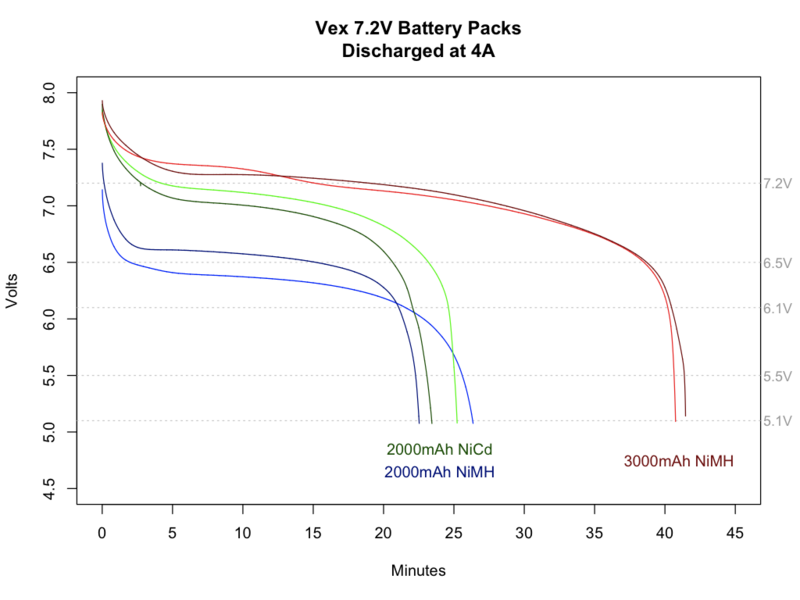
\includegraphics[width=\textwidth,height=8cm,keepaspectratio=true]{DischargeGraph}
    \caption{
        The VEX battery's discharge curve over various currents, thanks to Quazar \cite{Quazar}. Notice how the voltage virtually levels out during the majority of its lifetime; This makes it difficult to get an approximate percent throughout the entire lifetime of the battery with just voltage without using integration.
    }
\end{figure}

These complex methods are needed because the formula for a battery's discharge curve, for our battery's chemistry, is closer to a weird polynomial rather than linear or quadratic. I tried to get a cubic regression line for the discharge curves, but it fit it pretty badly and gave off results.

In the end, I simply turned the Arduino into a voltmeter that tells me whether or not the battery was near or at full capacity, and made a crummy percent bar that is only accurate through 100-90\% and 20-0\%; This was inspired by how another team, Renegade Robotics \cite{RenegadeRobotics}, does it.
